\subsection{Conceptual Description}
\label{sub:approach_conceptual_description}

\textbf{Architecture.} Figure~\ref{fig:stack} shows the \APIName stack. On the bottom layer are the \textit{Application layer protocols}. The Zeroconf protocols \textit{mDNS} and \textit{DNS-SD} are used for the advertisement and discovery of \APIshort services in the local network\footnote{We do not use these protocols directly but rely on their implementation in \textit{FlyWeb}.}. In terms of application-level network communication we use the common protocols of \textit{WebSocket} and \textit{HTTP}. The initial request to a \APIshort app is in form of a \textit{HTTP GET} request and associated request for static resources. Clients then establish a stable \textit{WebSocket} channel that is used for further communication between nodes (e.g. state replication). Above the application layer protocols is the \textit{FlyWeb} layer. We use FlyWeb as a library for facilitating interaction with the Zeroconf protocols. \APIName was designed with as few connection points with FlyWeb as possible such that this dependency can be easily replaced with a different implementation in the future. Above the FlyWeb layer is the \textit{\APIName} framework that exposes the API described in section~\ref{sub:approach_api_overview} to its applications that are located in the topmost layer.

\begin{figure}[h]
    \centering
    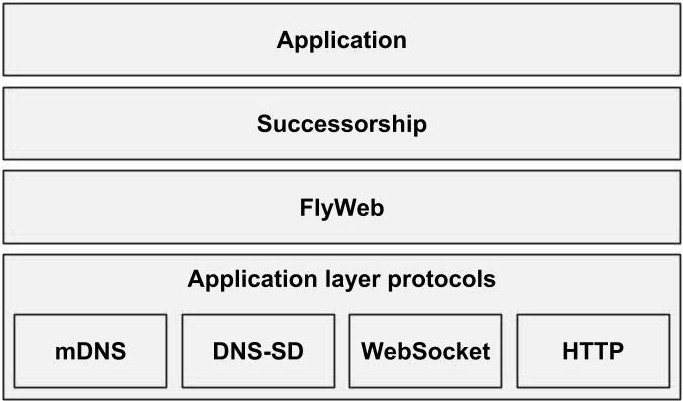
\includegraphics[width=\linewidth]{stack}
    \caption{Successorships Stack}
    \label{fig:stack}
\end{figure}



%Server publication and discovery
%Client Succession
%State Replication